\begin{figure*}
\centering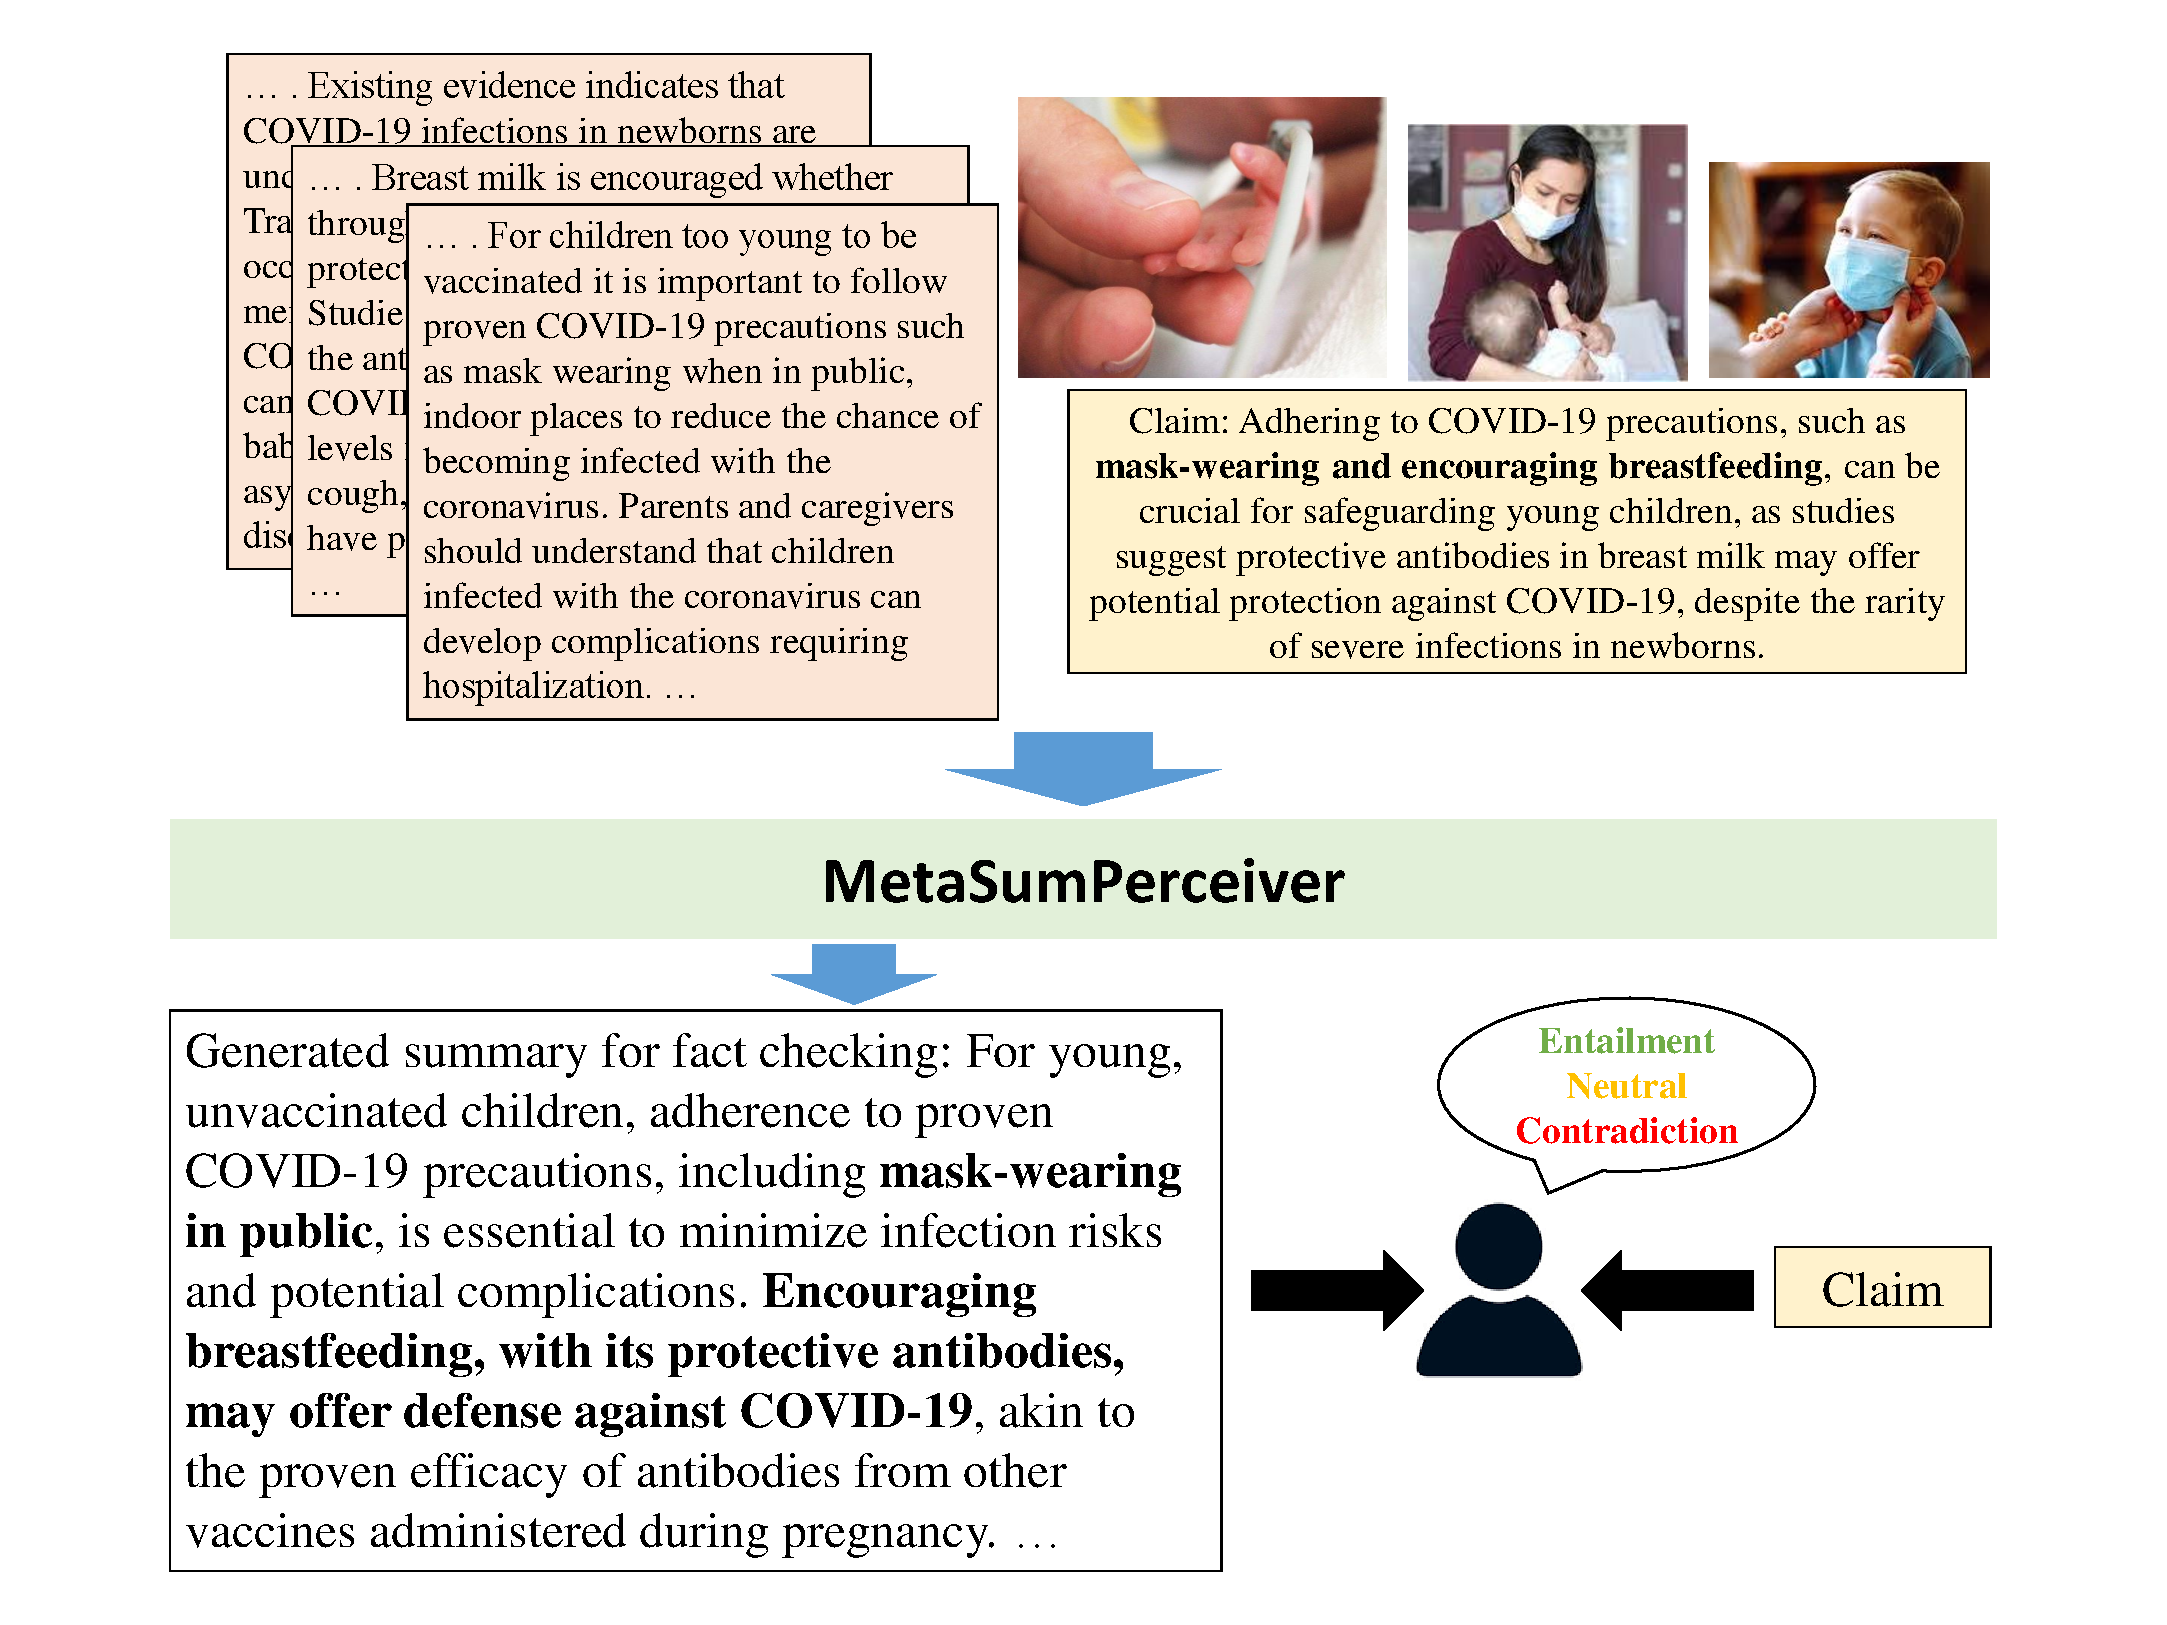
\includegraphics[width=\textwidth,height=0.5\textwidth,keepaspectratio]{images/metasumperceiver.pdf}
  \caption{Overview of MetaSumPerceiver: Using inputs such as documents, images, and claims, MetaSumPerceiver generates summaries to facilitate fact-checking. In this example, the summary for fact-checking provides evidence and establishes that the claim in question is entailed by the evidence.}
  \label{fig:metasumperceiver_overview}
\end{figure*}

To overcome the challenge of fact-checking with multimodal multi-document sources, we propose the~\textbf{MetaSumPerceiver} model in Figure~\ref{fig:metasumperceiver_overview}, where the input consists of a claim, a set of documents and images, and the objective is to generate a summary that expedites the fact-checking process for humans. we initially train the perceiver model~\cite{jaegle2022perceiver,jaegle2022perceiver_1} with a summarization model~\cite{lewis2019bart}. Subsequently, to produce the summary for fact-checking, we employ a proxy reward mechanism to update the summarizer to ensure the generation of an accurate and relevant summary with necessary evidence. Then, to train~\textbf{MetaSumPerceiver} to generate summaries useful for human fact-checking, we assess the utility of our summaries at performing entailment~\cite{inproceedings, poliak2020survey, bowman-etal-2015-large}, a closely aligned task to fact-checking. our work is orthogonal to prior work in entailment, in that rather than learning to predict the entailment label for the premise-hypothesis pair, we seek to generate the premise for a specific claim from a pool of multimodal data. In order to support research on the task of multimodal multi-document fact-checking, we also introduce the~\textbf{KG2Claim} approach outlined in Figure~\ref{fig:amrkg2claim}. This approach takes a multimodal multi-document knowledge graph as input and aims to create claims that incorporate this diverse information through multimodal coreference resolution~\cite{otmazgin2022fcoref, cattan2021realistic, caciularu-etal-2021-cdlm-cross}. 

\begin{figure*}
\centering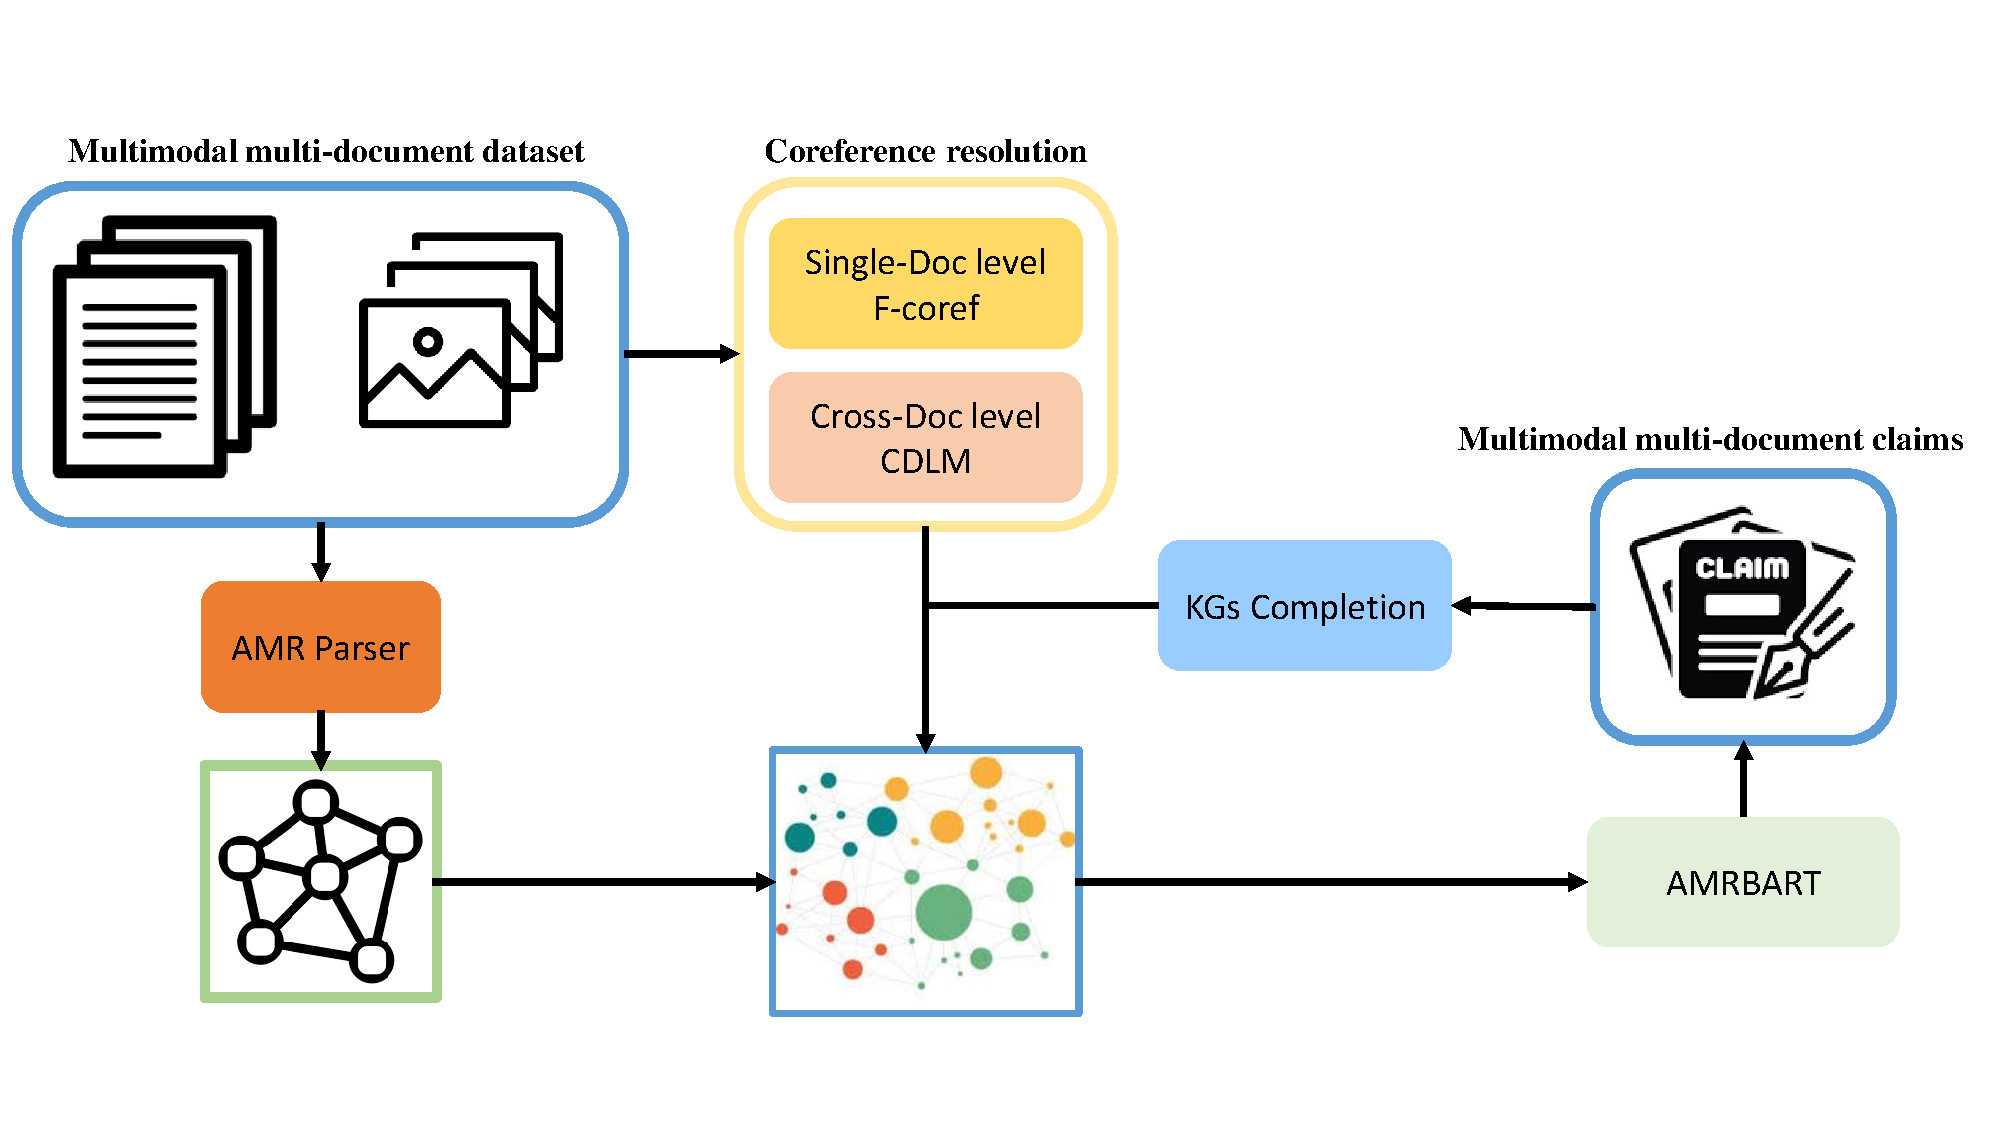
\includegraphics[width=\textwidth,height=0.5\textwidth,keepaspectratio]{images/amrkg2claim.pdf}
  \caption{Pipeline of KG2Claim: The elements encompass an AMR parser, single-document and cross-document coreference resolution, Knowledge graphs completion with LLMs, and AMRBART, generating the multimodal multi-document claims.}
  \label{fig:amrkg2claim}
\end{figure*}

To assess the efficiency of the~\textbf{MetaSumPerceiver}, we employ our~\textbf{KG2Claim} method for the fact-checking task, evaluate it against the MOCHEG benchmark~\cite{Yao_2023}, and introduce a new benchmark called Multi-News-Fact-Checking. Multi-News-Fact-Checking benchmark involves claims and entailment labels supported by evidence from multiple documents. Our results indicate significant enhancements compared to existing baselines.

The major contributions of this thesis are as follows:
\begin{itemize}
  
    \item We present an innovative approach for multimodal multi-document summarization specifically designed for fact-checking applications.

    \item We introduce a claim generation method tailored for disinformation detection tasks, with a focus on handling multimodal multi-document information.

    \item We release the Multi-News-Fact-Checking dataset, to support the multi-document fact-checking summarization task.
  
    \item We perform detailed experiments and ablations of our approach and loss functions which clearly demonstrate the superiority of our approach over existing methods.
  
\end{itemize}